\documentclass{article}
\usepackage{tikz}
\begin{document}
\begin{tikzpicture}
    \draw (0,0) -- (0,10) -- (10,10) -- (10,0) -- (0,0);
    \filldraw (0,0) circle (2pt) node[anchor=north]{$(x_1,y_1) = (0,0)$};
    \filldraw (10,10) circle (2pt) node[anchor=south]{$(x_2,y_2)=(0,0)$};
    
\end{tikzpicture}
\pagebreak


	
	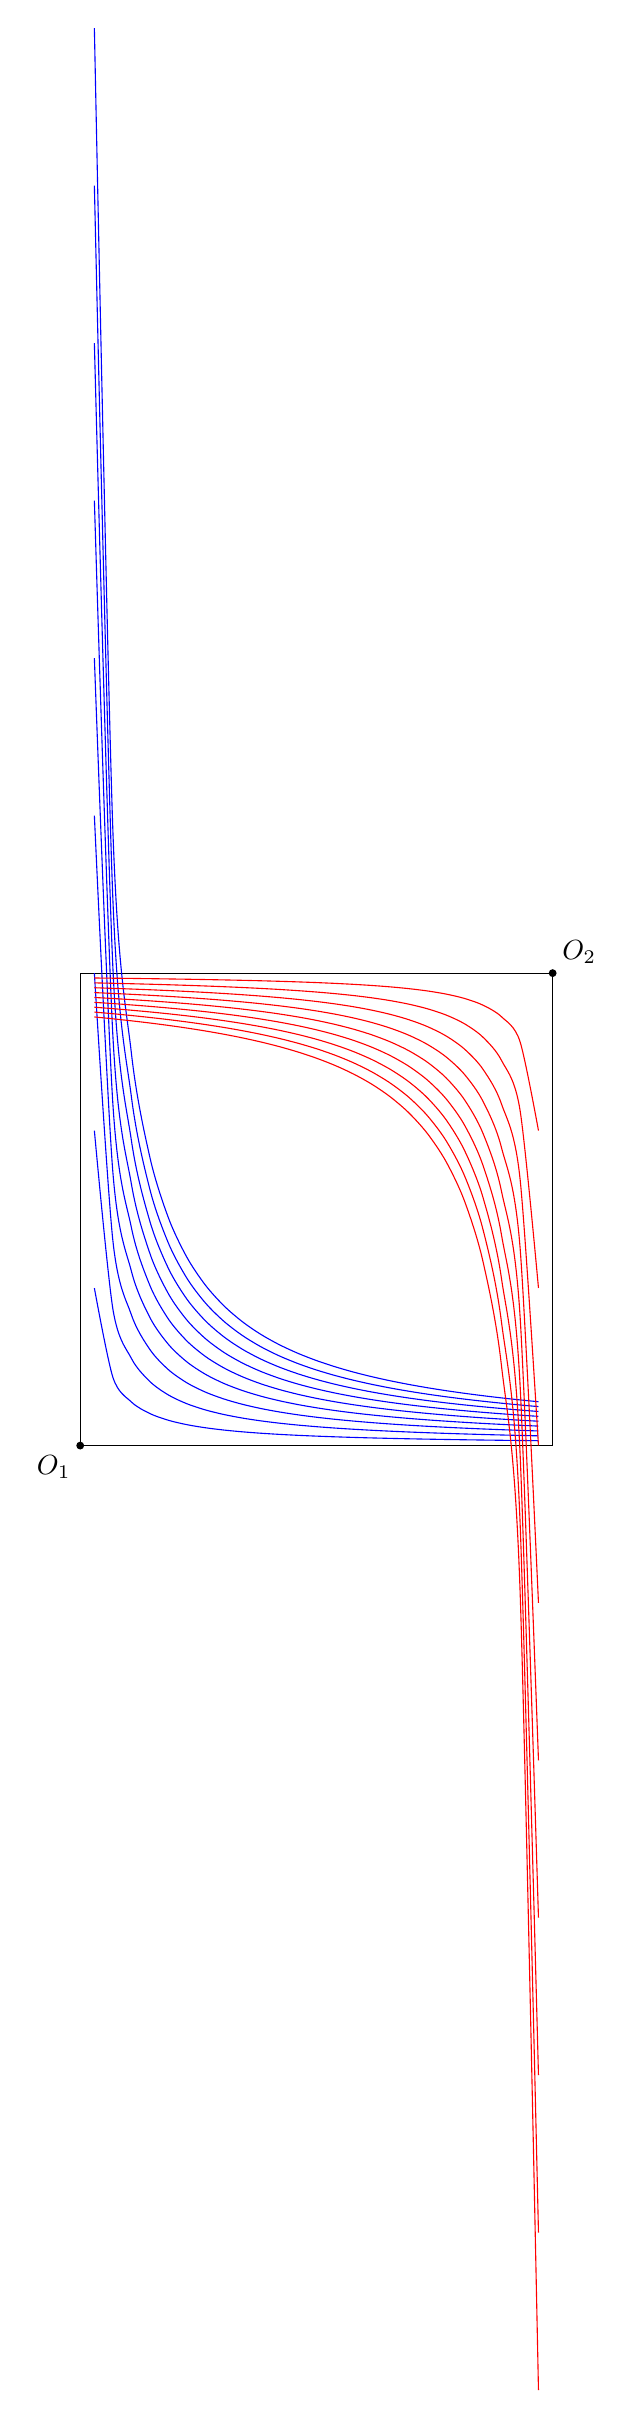
\begin{tikzpicture}[scale=0.6]
		
		% Box
		\draw (0,0) rectangle (10,10);
		
		% Origins
		\filldraw (0,0) circle (2pt) node[anchor=north east] {$O_1$};
		\filldraw (10,10) circle (2pt) node[anchor=south west] {$O_2$};
		
		% Consumer 1 indifference curves
		\foreach \k in {1,2,...,9} {
			\draw[blue, domain=0.3:9.7, smooth, variable=\x]
			plot ({\x}, {\k/(\x)});
		}
		
		% Consumer 2 indifference curves
		\foreach \k in {1,2,...,9} {
			\draw[red, domain=0.3:9.7, smooth, variable=\x]
			plot ({\x}, {10 - \k/(10-\x)});
		}
		
	\end{tikzpicture}
	
\pagebreak
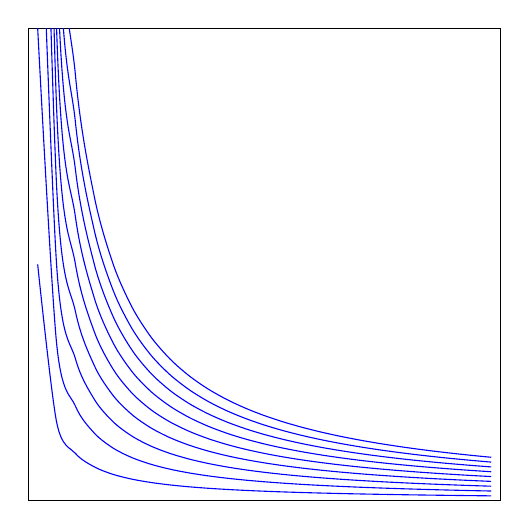
\begin{tikzpicture}[scale=0.6]
	
	\draw (0,0) rectangle (10,10);
	\clip (0,0) rectangle (10,10);
	
	\foreach \k in {1,2,...,9} {
		\draw[blue, domain=0.2:9.8, smooth, variable=\x]
		plot ({\x}, {\k/(\x)});
	}
	
\end{tikzpicture}
\end{document}